\section{Benchmark Results for the Onset of Rising Tone Chorus}
\label{sec:code}
We proceed with a series of simulations, employing our method to investigate the initiation of the whistler-mode chorus. The instability of the whistler wave typically arises from the electron temperature anisotropy instability \cite{kennel1966a,kennel1966b}, and the growth rate can be derived from the linear resonance condition near $\Omega \approx 0$.

In our simulation, the energetic electron distribution is bi-Maxwellian at the magnetic equator. 
Moving away from the magnetic equator, the equilibrium distribution maintains the similar form as it does in the phase space by conventional coordinates $(s_i, p_\|, \phi, \varphi)$. The distribution function in new canonical variables is given directly by canonical transfomation in ref \cite{zheng2023a}, and we have 
\begin{equation}
    \begin{aligned}
        & f_{0}(\Omega, \mathcal{J}) =\frac{\omega_{c e 0}}{(2 \pi)^{3 / 2} v_{t h \perp 0}^2 v_{t h \| 0}} \frac{1}{1-\beta} \cdot \exp \left(-\frac{k_l^2(\Omega+\Pi_i)^2}{2 v_{t h \| 0}^2}\right) \\
        &\cdot\left(\exp \left(-\frac{(\mathcal{J}+\Omega+\Pi_i) \omega_{c e 0}}{v_{t h \perp 0}^2}\right)-\exp \left(-\frac{(\mathcal{J}+\Omega+\Pi_i) \omega_{c e 0}}{\beta v_{t h \perp 0}^2}\right)\right)~,
        \end{aligned}
\end{equation}
where $\beta$ is the depth of the loss cone, the subscript $0$ denotes the magnetic equator.

As a realistic model for the magnetosphere, the magnetic field can be approximated as a dipole field, and the major component of the background magnetic field near the equator can be approximately represented by a parabolic function \cite{tao_numerical_2014}
\begin{equation}
    B(\lambda) = B_0(1+ R_a \lambda ^2)~,
\end{equation}
where $R_a$ is the inhomogeneity ratio of the magnetic field, $B_0$ is the magnetic field strength at the equator, and $\lambda$ is the magnetic latitude. The distance alone the magnetic field line $s$ satisfies $s = L R_E \lambda$.
The background electron density is found to fit a power law form \cite{denton2004},
\begin{equation}
    n(\lambda) = n_0 (1+R_b \lambda^2)~
\end{equation}
where $R_b$ is a fitting parameter in an order of one.

\subsection{Simulation configuration}
In conventional PIC simulations, the inhomogeneity ratio $R_a$ was often enlarged by one or two order of magnitudes to reduce the simulation cost.
However, one of the advantages of our numerical scheme is that we can use realistic parameters for the Earth's dipole field.
The basic parameters of our simulation are given in Tab. (\ref{tab.parameters}).
\begin{table}\label{tab.parameters}
    \centering
    \caption{Magnetic field and plasma parameters used in the simulation.\newline}
    \begin{tabular}{lc}
    \hline
     L-shell of the magnetic field line  & 5 \\
     Magnetic field inhomogeneity ratio $R_a$ &  4.5 \\
     Background cold plasma density inhomogeneity ratio $R_b$ &  1.0 \\
     Background electron gyro frequency and plasma frequency & \makecell{ $\omega_{ce} = 0.2$\\$\omega_{pe} = 1$  }\\
     Density ratio between energetic and cold  electrons at the magnetic equator &  0.002 \\
     Parallel and perpendicular thermal velocity of energetic electrons & \makecell{$v_\perp = 0.3 c$\\ $v_\| = 0.15c$}  \\
    Depth of the loss cone $\beta$ & 0 \\
    Size of the simulation domain  & \makecell{$\lambda \in [-15^\circ, 15^\circ]$ \\ $s \in [-6115,6115] c/\omega_{pe}$} \\
    \hline
    \end{tabular}\\
    \end{table}
%(useless) Note that, since we apply the electron plasma frequency $\omega_{pe0}$ at the equator for time normalization, the value always be 1 desites the L-shell value, which gyrofrequency is dynamcally changes.
The profile of the background parameter is shown in Fig. \ref{fig.profile}.
    \begin{figure}[htbp]
        \centering
        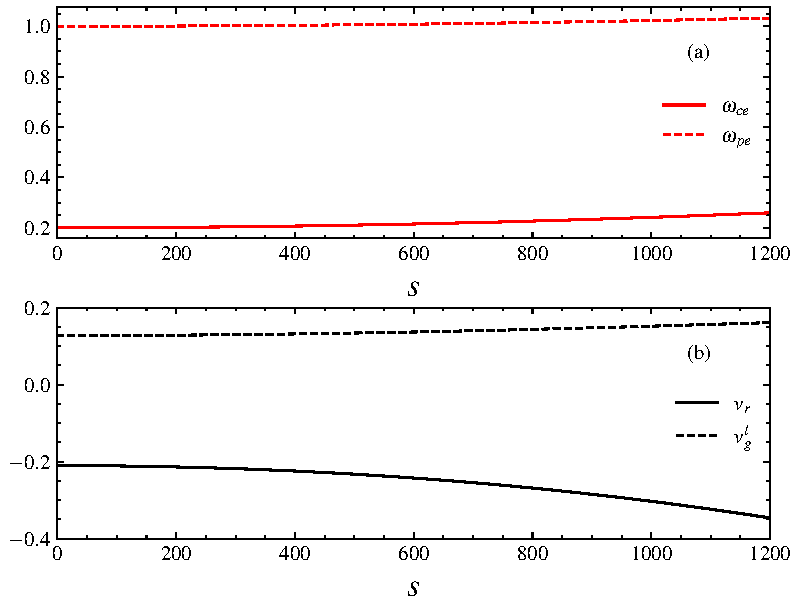
\includegraphics[scale=0.5]{cpc_img/fig_profile.pdf}
        \caption{(a) Background magnetic field and density profile. (b) Characterastic velocity in our simulation.}
        \label{fig.profile}
    \end{figure}
Meanwhile, we show the most unstable wave frequency applied in the simulation for the determination of initial reference frame. According to the choosen parameter in Tab. (\ref{tab.parameters}) and the definition of growth rate  $\gamma_l$ at the equator
\begin{equation}
\begin{aligned}
    \gamma_l(s) & =\frac{\sqrt{2 \pi} \omega_{c e} v_g \omega_{h 0}^2}{4 k_l^2 v_{t h \| 0}} e^{-\frac{\left(\omega_l-\omega_{c e}\right)^2}{2 k_l^2 v_{t h \| 0}}}
    \cdot \left((1+\beta) \frac{T_{\perp 0}}{T_{\| 0}} \frac{\omega_{c e 0}-\omega_l}{\omega_{c e 0}}-1\right)
    \end{aligned}
\end{equation}
The most unstable frequency is $\omega_l = 0.061$ and the corresponding growth rate is $\gamma_l \simeq 3.24\times 10^{-4}$, as shown by a scan of the parameter given in Fig.~\ref{fig.para}.
\begin{figure}[htbp]
    \centering
    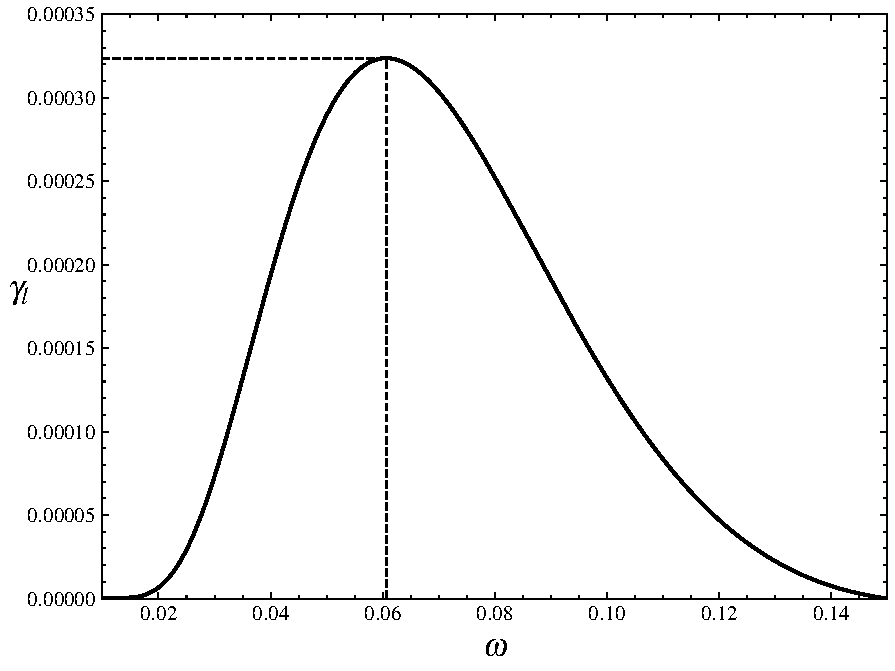
\includegraphics[scale=0.5]{cpc_img/fig_gamma1d.pdf}
    \caption{Linear growth rate $\gamma$ with respect to $\omega$ in the chosen parameter. The initial frequency of the wave is obtained from the most unstable frequency indicated by the vertical black line.}
    \label{fig.para}
\end{figure}

Benefiting from the scale-separated numerical scheme we set the number of grids for wave solver to 1001, aligning it with the number of sampling points in $s$.
In the $\mathcal{J}$ dimension, we employ a delta function, necessitating only a single sampling point for $\mathcal{J}$. In the case of a non-delta distribution, tens of sampling points prove sufficient for $\mathcal{J}$ sampling.
As to the $\xi,\Omega$ domain, the Eulerian grids are $31 \times 401$ for $\xi \in [0,2\pi]$ and $\Omega \in [-0.1,0.1]$.

The wave is resolved within a reduced-dimensional space, leading to a relatively manageable workload, as is the case with the Lagrangian solver. However, the bottleneck occurs within the Eulerian solver, primarily due to its two-dimensional space, necessitating hundreds of iterations for a single Lagrangian time step for all markers. Nonetheless, the computational cost remains reasonable in comparison to conventional PIC simulations, where the number of sampling points is at least several orders of magnitude greater than in our method. Consequently, their simulations require several billion particles \cite{nogi2022,katoh2016}, but the phase space resolution is significantly lower than ours.

\subsection{Benchmarks results}
The linear physics are quantitatively verified in Fig. \ref{fig.linear}, where we calculate the growth rate and the velocity of the maximum wave amplitude location before nonlinear effects become dominant. In the case of the propagating wave, we determine the trajectory of the wave packet using the integral of the group velocity,
\begin{equation}
    s(t) = s(0) + \int_0^{t} v_g(s(\tau)) \mathrm{d} \tau~.
\end{equation}
Here we trace the movement of the maximum amplitude point. Its propagation is in accord with the linear group velocity, as shown in Fig. \ref{fig.linear}(a). 
For the wave peak, it indeed propagates in the linear group velocity during the linear stage.
Moreover, we estimate the amplitude growth of the wave peak along its propagation path, the growth rate is given by \cite{nogi2022}
\begin{equation}\label{eq.gm_ver}
        \Gamma = \frac{1}{t_1-t_0}\log\frac{|a(s_1,t_1)|}{|a(s_0,t_0)|}~,
\end{equation}
where $s_0,t_0$, $s_1,t_1$ are along the prppagation path.
The growth of the amplitude along the propatation path is shown in Fig. \ref{fig.linear}(b). The corresponding growth rate from equation (\ref{eq.gm_ver}) is $\Gamma_0 \simeq 3.21\times10^{-4}$, agrees well with the theoretic linear growth rate shown in Fig. \ref{fig.para}.
The results show the correctness of our simulation at linear stage.
\begin{figure}[htbp]
    \centering
    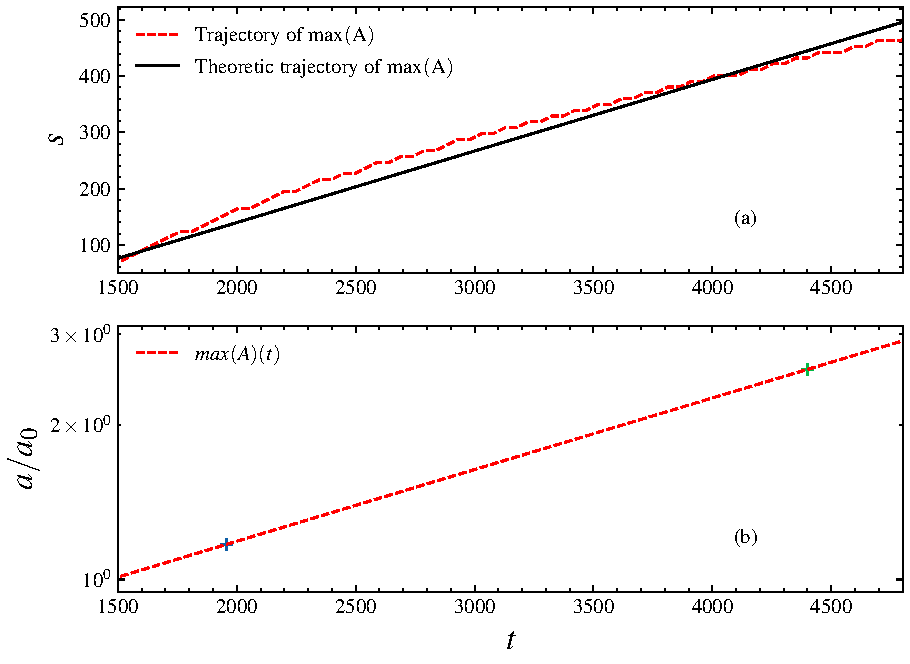
\includegraphics[scale=0.5]{cpc_img/fig_linear.pdf}
    \caption{Figure (a) is the propagation velocity of the linear wave packet with the maximum amplitude. Figure (b) denotes the growth of the wave peak amplitude with time along wave propagation path. The green cross marks the point used to caluclate the growth rate.}
    \label{fig.linear}
\end{figure}

In the nonlinear stage, trapped electrons form a phase space hole in $\xi-\Omega$. This phase space hole contributes to the nonlinear current, which in turn triggers the nonlinear frequency-chirping chorus wave. 
%The Hamiltonian for the resonant electrons has the form \cite{}
%\begin{equation}
%H = \frac{k^2\Omega^2}{2} + \frac{\omega_b^2}{k^2}\left(\cos \xi + \alpha \xi \right)~,
%\end{equation}
For the trapped electrons, it fells an osillatory force from the wave and a noninertial force from background inhomogeneity. The forces can be described by a potential well with the form $\sin \xi + \alpha \xi$, with parameter $\alpha$ as an inhomogeneity ratio \cite{omura2008,tao2020}
\begin{equation}\label{eq.alp}
    \alpha \equiv \frac{1}{\omega_{b}^2}\left[\left(1 - 2\frac{v_r}{v_g}\right)\frac{\partial \omega}{\partial t}  -v_r^2 \frac{\partial k}{\partial s}+ \frac{\mathrm{\partial} \omega_{ce}}{\mathrm{\partial} s}\frac{k_i}{m_e}\mathcal{J}\right].
\end{equation}
From the potential well, we can find the X point of the phase space trajectory, i.e., the inflection point of the potential well
\begin{equation}
    \xi_\mathrm{x} = - \arcsin \alpha,
\end{equation}
and the C point of the trajectory is obtained from the energy on the separatrix $e_\mathrm{spx} = \sin \xi_\mathrm{x} + \alpha \xi_\mathrm{x}$,
\begin{equation}
    \sin \xi_\mathrm{c} + \alpha \xi_\mathrm{c} = e_\mathrm{spx}.
\end{equation}
The shape of the hole, specifically its boundary, can be analytically described as follows \cite{zheng2023a,omura2008}:
\begin{equation}\label{eq.Omega_b}
    \Omega(\xi) = \pm \frac{\omega_b}{k^2} \sqrt{2 (e_\mathrm{spx}-\cos \xi - \alpha \xi)}~,
\end{equation}
where $k$ is the wave number and $\omega_b\equiv \sqrt{k^2 v_\perp a}$ is the trapped particle bounce frequency and


In Fig.~\ref{fig.hole}, we present a typical electron phase-space hole observed at a specific location $s$ in the late nonlinear stage. We determined the corresponding values of $k \simeq 0.649$, $\omega_b \simeq 0.007$, $\alpha \simeq 0.08$ based on the simulation data at that location. Additionally, we illustrated the boundary of the hole using the equation (\ref{eq.Omega_b}). Notably, the shape of the hole closely aligns with the theoretical predictions.

\begin{figure}[htbp]
    \centering
    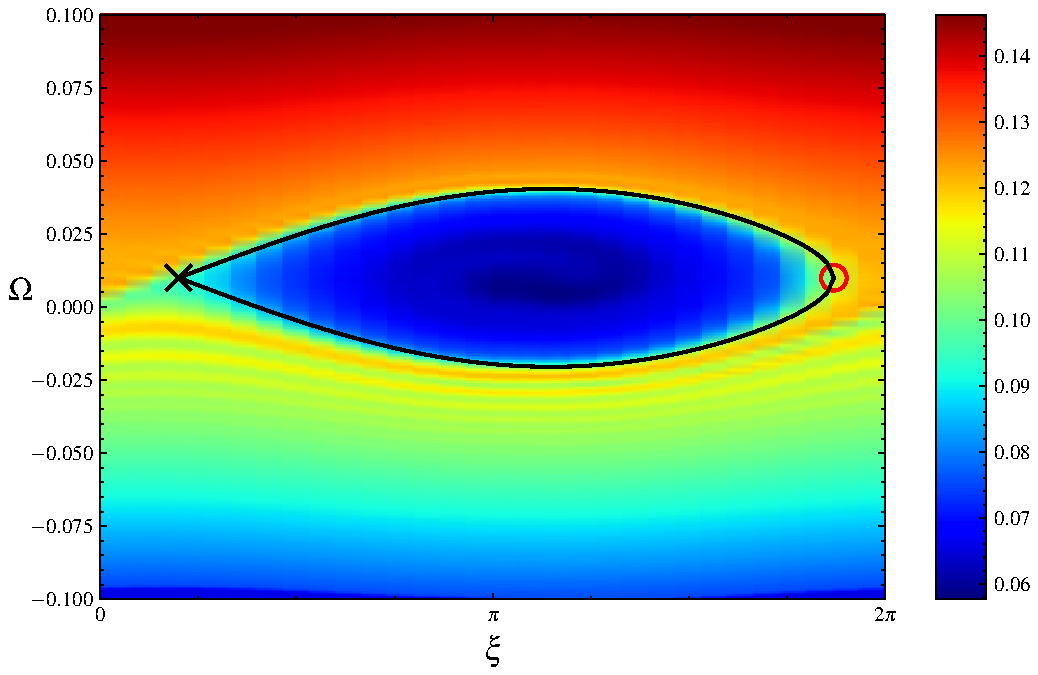
\includegraphics[scale=0.5]{cpc_img/fig_hole.pdf}
    \caption{Phase-space hole  formed by trapped electrons at $s\simeq 2107$ in the wave field. The X, C points on the left and right ends and the boundary of the hole are obtained from theory.}
    \label{fig.hole}
\end{figure}


